\documentclass[conference]{IEEEtran}

\usepackage[T1]{fontenc}
\usepackage[utf8]{inputenc}
\usepackage{cite}
\usepackage{amsmath}
\usepackage{graphicx}
\usepackage{booktabs}
\usepackage{xcolor}
\usepackage{tikz}
\usetikzlibrary{arrows.meta, positioning}
\usepackage{url}

\begin{document}

\title{Multilingual Sentiment Analysis with System One Models}

\author{
\IEEEauthorblockN{Uran Laj\c{c}i\IEEEauthorrefmark{1}\IEEEauthorrefmark{2},
Zenun Kastrati\IEEEauthorrefmark{3},
Lule Ahmedi\IEEEauthorrefmark{1} and
Kadri Sylejmani\IEEEauthorrefmark{1}\IEEEauthorrefmark{4}}
\IEEEauthorblockA{\IEEEauthorrefmark{1}Faculty of Electrical and Computer Engineering, University of Prishtina, Bregu i Diellit p.n., Prishtinë, 10000, Kosovë}
\IEEEauthorblockA{\IEEEauthorrefmark{2}Care Software, Prishtinë, 10000, Kosovë}
\IEEEauthorblockA{\IEEEauthorrefmark{3}Department of Informatics, Linnaeus University, Växjö, Sweden}
\IEEEauthorblockA{\IEEEauthorrefmark{4}Center for Artificial Intelligence, University of Prishtina, Prishtinë, 10000, Kosovë}
\IEEEauthorblockA{uran.lajqi@uni-pr.edu, zenun.kastrati@lnu.se (corresponding author), lule.ahmedi@uni-pr.edu, kadri.sylejmani@uni-pr.edu}
}

\maketitle

\begin{abstract}
Large language models (LLMs) classify sentiment well without training, but they are costly to run at scale and weaker on low-resource languages. System One models do not generate text: they answer typed questions with a probability for each option. We compare three System One models, Jev, Clef and Clef-flash, with the five LLMs evaluated by Kastrati et al.\ on three-class sentiment analysis in eight languages, on the same 12,970 test items. Zero-shot, Jev reaches a mean macro-F1 of 61.7 and ranks third of the eight models, behind Claude 3.7 Sonnet and GPT-4o. The LLMs' few-shot examples help every LLM but none of the System One models. We then let Claude Opus 5.5 write Jev's question from labelled train data and tune it on Jev's errors, and we select the final question on validation data that Opus never sees. With the tuned question, Jev's mean rises to 67.4, and it reaches the best score of all models on German, Albanian, Bosnian and Croatian. On Swedish, the one language with reported LLM costs, zero-shot Jev cost less than every LLM, and tuned Jev less than GPT-4o, Claude and Mistral, after a one-time tuning of US\$2 to US\$17 per language.
\end{abstract}

\begin{IEEEkeywords}
sentiment analysis, System One models, large language models, low-resource languages, prompt optimization
\end{IEEEkeywords}

\section{Introduction}
Sentiment analysis of social media posts helps to follow public opinion on health, politics and products. Large language models (LLMs) now classify sentiment well without task-specific training, but their quality is uneven across languages. Kastrati et al.~\cite{kastrati2026language} evaluated five LLMs on 36 sentiment datasets and found them clearly weaker on low-resource languages. LLMs are also costly to run over millions of posts, because each text needs a full generation call.

System One models offer another interface. They do not generate text: they answer typed questions about an input, such as a choice among fixed options, and return a probability for each option~\cite{typesafe2026jev}. Jev, the first such model, answered 346,009 benchmark requests for under US\$10~\cite{deusser2026jev}. On sentiment and emotion tasks, however, plain Jev still trails the strongest LLMs~\cite{zhang2026emojev}. Two questions remain open. How do System One models compare with LLMs on multilingual three-class sentiment analysis, on the same test items? And can a better question close the gap, since a System One model is adapted only through its question?

This paper answers both questions on eight languages and 12,970 test items, against the five LLMs of Kastrati et al. Our contributions are:
\begin{itemize}
\item a zero-shot and few-shot evaluation of three System One models, Jev, Clef and Clef-flash, on the test items that Kastrati et al. scored;
\item a method in which an LLM, Claude Opus 5.5, writes Jev's question from labelled train data and tunes it on Jev's errors, with the final question selected on validation data that the LLM never sees;
\item results showing that zero-shot Jev ranks third of eight models, that the LLMs' few-shot examples do not help System One models, and that tuned Jev reaches the best score of all models on four of the eight languages, after a one-time tuning that cost US\$2 to US\$17 per language.
\end{itemize}

\section{Related Work}
\textit{Multilingual sentiment analysis.} Fine-tuned multilingual encoders such as XLM-T~\cite{barbieri2022xlmt} set strong baselines on tweets in many languages, and dedicated models exist for low-resource languages such as Albanian~\cite{kastrati2021albana}. Kastrati et al.~\cite{kastrati2026language} instead prompted five LLMs, zero-shot and few-shot, on 36 datasets from several language families. Few-shot examples helped most languages, but low-resource languages stayed clearly behind. We reuse their test items and LLM scores, so our models are compared on exactly the same data.

\textit{System One models.} Deußer et al.~\cite{deusser2026jev} evaluated Jev zero-shot on 37 datasets. It beat Qwen3.8-27B on 27 of them and reached 86.7\% accuracy on Belebele across 122 languages, but it lost quality on low-resource languages and noisy labels. Zhang and Yu~\cite{zhang2026emojev} reported 62.93\% average macro-F1 for plain Jev on eight sentiment, emotion, sarcasm and humor datasets, against 67.28\% for the strongest LLM. They narrowed the gap by splitting the task into smaller judgments. Zhang et al.~\cite{zhang2026decide} decomposed aspect-based sentiment analysis into Jev decisions and reached the lowest valence--arousal error in SemEval-2026 Task~III, without generating text. None of these studies tests System One models on multilingual three-class sentiment against LLMs on the same items, and none lets an LLM write the questions.

\textit{Writing and tuning prompts with LLMs.} In instruction induction, an LLM writes a task description from a few labelled examples~\cite{honovich2023instruction}. Automatic Prompt Engineer~\cite{zhou2023ape} generates many candidate instructions and keeps the one with the best score. ProTeGi~\cite{pryzant2023protegi} improves a prompt step by step from the errors it causes. Our method follows the last two ideas for a model that does not generate text: the LLM rewrites a typed question from Jev's errors on train data, and the version is chosen on validation data that the LLM never sees.

\section{Data and Models}

\subsection{Datasets}
We use eight of the test sets of Kastrati et al.~\cite{kastrati2026language}, with exactly the items they scored (Table~\ref{tab:datasets}). English, German and French come from the Tweet Sentiment Multilingual collection~\cite{barbieri2022xlmt}, which draws 870 test tweets per language from SemEval-2017~\cite{rosenthal2017semeval}, SB-10K~\cite{cieliebak2017sb10k} and DEFT 2017~\cite{benamara2017deft}. The Albanian set is AlbAna, Facebook comments under posts of the National Institute of Public Health of Kosovo during the COVID-19 pandemic~\cite{kastrati2021albana}. The Bosnian, Croatian, Serbian and Swedish sets are tweets labelled by native speakers~\cite{mozetic2016multilingual,mozetic2018evaluate}; for the first three, the test sets are the 20\% samples of Kastrati et al. We chose these eight languages because each has train and validation data, which the tuned questions need. Together, the test sets hold 12,970 items.

For the three Tweet Sentiment Multilingual languages, we use the collection's own train and validation splits. For the other five, we split the items outside the test sample into 80\% train and 20\% validation, stratified by label. In all eight, we removed every train and validation text that also occurs in the test set. Every item has one of three labels: positive, neutral or negative. We report macro-F1 over the three labels, as Kastrati et al. do.

\begin{table}[t]
\centering
\caption{The eight datasets. The Albanian texts are Facebook comments. Test is the sample that Kastrati et al.~\cite{kastrati2026language} scored; train and validation exclude every test item.}
\label{tab:datasets}
\setlength{\tabcolsep}{3pt}
\begin{tabular}{llrrrr}
\toprule
Language & Source & Text & Test & Train & Valid. \\
\midrule
English & SemEval-2017~\cite{rosenthal2017semeval,barbieri2022xlmt} & tweets & 870 & 1,839 & 324 \\
German & SB-10K~\cite{cieliebak2017sb10k,barbieri2022xlmt} & tweets & 870 & 1,839 & 324 \\
French & DEFT 2017~\cite{benamara2017deft,barbieri2022xlmt} & tweets & 870 & 1,837 & 323 \\
Albanian & AlbAna~\cite{kastrati2021albana} & comments & 2,148 & 6,819 & 1,705 \\
Bosnian & Mozeti\v{c} et al.~\cite{mozetic2016multilingual} & tweets & 782 & 27,949 & 6,988 \\
Croatian & Mozeti\v{c} et al.~\cite{mozetic2016multilingual} & tweets & 2,790 & 57,624 & 14,406 \\
Serbian & Mozeti\v{c} et al.~\cite{mozetic2016multilingual} & tweets & 2,272 & 52,263 & 13,066 \\
Swedish & Mozeti\v{c} et al.~\cite{mozetic2016multilingual} & tweets & 2,368 & 32,205 & 8,052 \\
\bottomrule
\end{tabular}
\end{table}


\subsection{Models}
System One models do not generate text. They answer typed questions about an input, which TypeSafe calls the state~\cite{typesafe2026jev,deusser2026jev}. A Choice question has instructions and one criterion per option, and the model returns a probability for each option. We test three such models. Jev (\texttt{jev-1.14.0}) is a commercial model from TypeSafe AI~\cite{typesafe2026jev}. Clef and Clef-flash are open-weight models from Cloudflare, fine-tuned from Qwen3.8-27B and Qwen3.5-9B, which we call through Cloudflare Workers AI~\cite{cloudflare2026clef} at Hugging Face revisions \texttt{cfddda0} and \texttt{fb4417d}. We pin every version so that the results can be reproduced.

The LLM baselines are the five models that Kastrati et al.~\cite{kastrati2026language} evaluated with one shared prompt: GPT-4o (\texttt{gpt-4o-2024-08-06}), Gemini 2.0 Flash, DeepSeek-V3, Mistral Large (\texttt{mistral-large-2411}) and Claude 3.7 Sonnet. We take their zero-shot and few-shot scores from that paper; we did not run the LLMs ourselves.

\section{Method}

\subsection{Zero-shot question}
All three models get one Choice question, written in English and the same for every language. Its instructions ask for the overall sentiment that the author of the text expresses. Each label has a one-sentence criterion, such as ``The text expresses a positive opinion, emotion or attitude'' for positive.

\subsection{Few-shot question}
The few-shot question adds the three English examples that Kastrati et al.~\cite{kastrati2026language} gave the LLMs, one per label. Each criterion becomes an object that holds the zero-shot description and the example for that label. The input therefore differs in one way from the LLMs': they saw the examples before the text, while our models see them inside the criteria.

\subsection{Tuned question}
For Jev, we also let an LLM write and tune the question from labelled train data (Fig.~\ref{fig:tuning}). The method combines instruction induction~\cite{honovich2023instruction}, in which an LLM writes a task description from labelled examples, with prompt optimization from error feedback~\cite{pryzant2023protegi}. Claude Opus 5.5 (\texttt{claude-opus-5-5}, effort \texttt{medium}) performs both steps.

\textit{Input.} The state holds the text and a context of one to three sentences that we wrote from each dataset's paper: its source, time and language. For Albanian, for example, it begins ``A Facebook comment under a post by the National Institute of Public Health of Kosovo during the COVID-19 pandemic in 2020.'' The instructions hold a question and a rule that says where the annotators draw the line between the labels. Each criterion holds a description of the label, one to four train texts as examples with their English meaning, cue words, and the texts that look like the label but get another one. Jev gets this question three times in one request, with the labels in three rotated orders, and we average the three probabilities, because Jev leans toward the first option.

\textit{Start question.} Opus reads the context and 150 train texts, 50 per label, and writes the question in this format, in at most 400 words.

\textit{Tuning loop.} We draw a development set of 600 other train texts, which keep the train label proportions. Jev scores the current version on the development and validation sets, with one label order to save cost. Opus receives the development macro-F1, the confusion matrix and every misclassified text with its gold label, Jev's label and Jev's probabilities. It writes an error analysis and then the next version. After ten rewrites, we keep the version with the highest validation macro-F1. Opus never sees validation data, so it cannot fit the selection set. Jev then scores the kept version once on the test set, with the three label orders averaged. We make one run per language.

A tuned question has thus used 750 labelled train texts and the validation set, while the LLMs saw three examples. We therefore compare it with the best score that any LLM reached on the language, zero-shot or few-shot.

\begin{figure}[t]
\centering
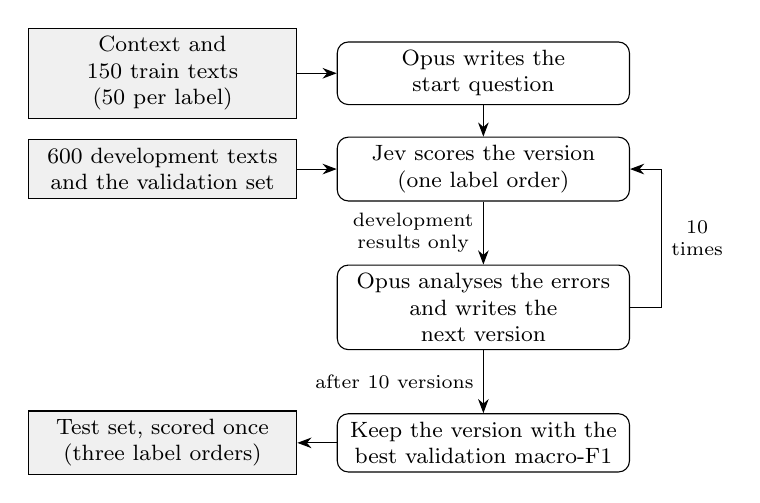
\begin{tikzpicture}[
  node distance=4mm and 5mm,
  action/.style={draw, rounded corners, align=center, font=\footnotesize, inner sep=3pt, text width=3.5cm},
  data/.style={draw, align=center, font=\footnotesize, inner sep=3pt, fill=gray!12, text width=3.2cm},
  arrow/.style={-{Stealth[length=1.8mm]}},
  tag/.style={font=\scriptsize, align=center}
]
\node[data] (train) {Context and 150 train texts\\(50 per label)};
\node[action, right=of train] (start) {Opus writes the\\start question};
\node[action, below=of start] (score) {Jev scores the version\\(one label order)};
\node[data, left=of score] (sets) {600 development texts\\and the validation set};
\node[action, below=8mm of score] (rewrite) {Opus analyses the errors\\and writes the next version};
\node[action, below=8mm of rewrite] (keep) {Keep the version with the\\best validation macro-F1};
\node[data, left=of keep] (test) {Test set, scored once\\(three label orders)};
\draw[arrow] (train) -- (start);
\draw[arrow] (start) -- (score);
\draw[arrow] (sets) -- (score);
\draw[arrow] (score) -- node[tag, left] {development\\results only} (rewrite);
\draw[arrow] (rewrite.east) -- ++(4mm,0) |- node[tag, right, pos=0.25] {10\\times} (score.east);
\draw[arrow] (rewrite) -- node[tag, left] {after 10 versions} (keep);
\draw[arrow] (keep) -- (test);
\end{tikzpicture}
\caption{Writing and tuning Jev's question for one language. Opus sees train data only; the validation set selects the version, and the test set is scored once.}
\label{fig:tuning}
\end{figure}

\section{Results}

\begin{table*}[t]
\centering
\caption{Macro-F1 (\%) of the three System One models and of the five LLMs reported by Kastrati et al.~\cite{kastrati2026language}, zero-shot and few-shot with the same three English examples. Bold marks the best score in each column of a block. The mean is unweighted over the eight languages.}
\label{tab:zero-few-shot}
\begin{tabular}{lrrrrrrrrr}
\toprule
Model & EN & DE & FR & SQ & BS & HR & SR & SV & Mean \\
\midrule
\multicolumn{10}{l}{\textit{Zero-shot}} \\
Jev & 68.0 & 73.3 & 63.7 & 58.2 & \textbf{59.2} & \textbf{56.9} & 52.5 & 61.4 & 61.7 \\
Clef & 64.9 & 65.9 & 39.9 & 55.4 & 48.0 & 40.1 & 49.7 & 68.7 & 54.1 \\
Clef-flash & 61.1 & 55.1 & 38.7 & 45.7 & 41.8 & 36.6 & 47.9 & 61.0 & 48.5 \\
\cmidrule(lr){1-10}
GPT-4o & 70.1 & 71.0 & 55.8 & \textbf{69.8} & 58.3 & 50.5 & \textbf{58.1} & \textbf{78.7} & 64.0 \\
Gemini & 65.1 & 61.4 & \textbf{64.9} & 53.4 & 54.6 & 55.1 & 50.1 & 72.9 & 59.7 \\
DeepSeek & 71.9 & 70.8 & 58.2 & 54.0 & 55.6 & 56.3 & 47.6 & 69.1 & 60.4 \\
Mistral & 62.5 & 60.9 & 51.7 & 50.3 & 43.8 & 37.6 & 45.9 & 66.4 & 52.4 \\
Claude & \textbf{73.3} & \textbf{75.6} & 52.6 & 64.8 & \textbf{59.2} & 53.5 & 57.1 & 76.7 & \textbf{64.1} \\
\midrule
\multicolumn{10}{l}{\textit{Few-shot}} \\
Jev & 68.7 & 74.4 & 62.4 & 58.2 & 59.6 & 56.9 & 53.4 & 62.4 & 62.0 \\
Clef & 53.5 & 58.6 & 29.1 & 46.8 & 41.1 & 33.5 & 46.0 & 62.9 & 46.4 \\
Clef-flash & 57.1 & 50.3 & 36.3 & 42.0 & 38.1 & 34.0 & 44.9 & 58.5 & 45.2 \\
\cmidrule(lr){1-10}
GPT-4o & 70.8 & 74.8 & 65.1 & \textbf{70.2} & 61.7 & 56.6 & \textbf{59.1} & \textbf{79.6} & \textbf{67.2} \\
Gemini & 66.4 & 68.6 & 63.2 & 70.0 & 61.2 & 53.3 & 56.3 & 76.1 & 64.4 \\
DeepSeek & 69.7 & 75.1 & 48.7 & 63.6 & 62.2 & 59.4 & 56.5 & 76.6 & 64.0 \\
Mistral & 68.4 & 76.0 & \textbf{66.3} & 53.8 & 61.3 & \textbf{63.5} & 51.8 & 78.5 & 65.0 \\
Claude & \textbf{72.4} & \textbf{77.2} & 63.0 & 65.4 & \textbf{64.4} & 61.9 & 54.5 & 75.5 & 66.8 \\
\bottomrule
\end{tabular}
\end{table*}


\subsection{Zero-shot}
Zero-shot Jev reaches a mean macro-F1 of 61.7 (Table~\ref{tab:zero-few-shot}). It ranks third of the eight models, behind Claude (64.1) and GPT-4o (64.0) and ahead of DeepSeek (60.4), Gemini (59.7) and Mistral (52.4). Jev is the best model on Croatian and ties Claude on Bosnian. Its largest gaps are on Swedish (61.4 against 78.7 for GPT-4o) and Albanian (58.2 against 69.8). Clef (54.1) and Clef-flash (48.5) score lower, mainly because they label 65\% and 73\% of the texts neutral, while only 34\% are neutral; Jev labels 27\% neutral.

\subsection{Few-shot}
The three examples raise the mean of every LLM, by 2.7 points for Claude up to 12.6 for Mistral. They do not help the System One models: Jev gains 0.3 points, while Clef loses 7.7 and Clef-flash 3.3. Clef and Clef-flash label even more texts neutral than in zero-shot (75\% and 77\%). With few-shot, Jev (62.0) falls below all five LLMs, which range from 64.0 to 67.2.

\begin{table}[t]
\centering
\caption{Macro-F1 (\%) of Jev zero-shot (ZS), few-shot (FS) and with the tuned question, against the highest score any of the five LLMs reached on that language, zero-shot or few-shot. Bold marks a tuned score above the best LLM score.}
\label{tab:tuned}
\setlength{\tabcolsep}{3pt}
\begin{tabular}{lrrrrlr}
\toprule
 & \multicolumn{3}{c}{Jev} & \multicolumn{2}{c}{Best LLM} & \\
\cmidrule(lr){2-4}\cmidrule(lr){5-6}
Language & ZS & FS & Tuned & Score & Model & $\Delta$ \\
\midrule
English & 68.0 & 68.7 & 70.6 & 73.3 & Claude ZS & $-2.7$ \\
German & 73.3 & 74.4 & \textbf{79.9} & 77.2 & Claude FS & $+2.7$ \\
French & 63.7 & 62.4 & 65.5 & 66.3 & Mistral FS & $-0.8$ \\
Albanian & 58.2 & 58.2 & \textbf{73.5} & 70.2 & GPT-4o FS & $+3.3$ \\
Bosnian & 59.2 & 59.6 & \textbf{68.7} & 64.4 & Claude FS & $+4.3$ \\
Croatian & 56.9 & 56.9 & \textbf{64.3} & 63.5 & Mistral FS & $+0.8$ \\
Serbian & 52.5 & 53.4 & 56.8 & 59.1 & GPT-4o FS & $-2.3$ \\
Swedish & 61.4 & 62.4 & 59.7 & 79.6 & GPT-4o FS & $-19.9$ \\
\midrule
Mean & 61.7 & 62.0 & 67.4 & 69.2 & & $-1.8$ \\
\bottomrule
\end{tabular}
\end{table}


\subsection{Tuned question}
The tuned question raises Jev's mean to 67.4, a gain of 5.7 points over zero-shot (Table~\ref{tab:tuned}). It helps on seven of the eight languages, from 2.6 points on English to 15.3 on Albanian. On German, Albanian, Bosnian and Croatian, tuned Jev beats the best score that any LLM reached in either setting, by 0.8 to 4.3 points. On French, Serbian and English it is 0.8 to 2.7 points behind, and on Swedish it is far behind. Its mean is slightly above the best LLM setting, few-shot GPT-4o (67.2), and below the mean of the best LLM score per language (69.2), which picks a different LLM for each language.

The gains come mostly from the neutral label, which the zero-shot question defines too narrowly for these annotators. On Albanian, where 57\% of the test comments are neutral, Jev's neutral recall rises from 0.50 to 0.77, and on German from 0.51 to 0.73. The tuned questions describe the annotators' conventions. The Albanian one, for example, makes neutral the default for questions, forecasts, policy complaints without blame words and jokes that rank cities by case counts, and keeps negative for curses, insults, explicit blame of the government and claims that the institute is lying.

\subsection{Cost and speed}
System One models charge per input token, and every request carries the whole question. Jev costs US\$0.042 per million input tokens. Zero-shot, it reads 385 tokens per text, which costs US\$0.02 per 1,000 texts; Clef and Clef-flash cost about US\$0.05 and US\$0.01. The tuned question is long and sent in three label orders, so it reads about 3,400 tokens per text, or US\$0.14 per 1,000 texts. Tuning is a one-time cost: US\$2.3 to US\$3.2 per language for English, German, French and Albanian, and US\$10 to US\$17 for Bosnian, Croatian, Serbian and Swedish, where Opus read longer error lists and Jev scored validation sets of 7,000 to 14,000 texts. All eight languages cost US\$64.

Kastrati et al.~\cite{kastrati2026language} report the API prices of the five LLMs, from US\$0.10 (Gemini) to US\$3.00 (Claude) per million input tokens, and the cost of their runs on a few datasets. Of our languages, only Swedish is among them. On its 2,368 test texts, their runs cost US\$1.48 for GPT-4o, US\$2.05 for Claude, US\$2.44 for Mistral, US\$0.11 for Gemini and US\$0.07 for DeepSeek. On the same texts, zero-shot Jev cost US\$0.04, less than every LLM, and tuned Jev cost US\$0.37. That is four to seven times less than GPT-4o, Claude and Mistral, but more than Gemini and DeepSeek. Jev also returns only probabilities: with 16 parallel requests, it answered about 34 texts per second with the tuned question in one label order. We did not measure the speed of the LLMs.

\section{Discussion and Limitations}
Our results suggest that a System One model is limited less by what it can judge than by how the question describes the labels. Zero-shot, Jev already competes with most LLMs, and a question that states each dataset's own conventions lifts it above all of them on four languages. The LLMs' few-shot examples do not have this effect: three English examples say little about where the annotators of a Bosnian or Albanian dataset draw the line between neutral and negative.

Swedish is the exception. Tuning barely changed the validation score (65.1 to 65.7), and the kept question scored 59.7 on test, below zero-shot Jev. The gap between validation and test is the largest of all languages, which suggests that the test sample differs from the rest of the dataset; we did not study why.

The study has four main limitations. First, we made one tuning run per language, so we do not know how much the tuned scores vary between runs; the differences of about one point between tuned Jev and the best LLM are within that unknown range. Second, the tuned questions use 750 labelled train texts and the validation set, while the LLMs saw three examples; LLMs given the same data and tuning might also improve. Third, we took the LLM scores from Kastrati et al.~\cite{kastrati2026language} rather than running the LLMs ourselves, so prompts, input formats and dates differ. Fourth, the models may have seen these public datasets during training, which we cannot check.

\section{Conclusion}
We compared three System One models with five LLMs on three-class sentiment analysis in eight languages, on the same 12,970 test items. Zero-shot, Jev ranks third of the eight models, while Clef and Clef-flash label too many texts neutral. The LLMs' few-shot examples help the LLMs but not the System One models. When Claude Opus 5.5 writes Jev's question from labelled train data and tunes it on Jev's errors, Jev's mean rises from 61.7 to 67.4, and it reaches the best score of all models on German, Albanian, Bosnian and Croatian. Future work will repeat the tuning with several runs, extend the study to all 35 languages of Kastrati et al., and tune the questions of other System One models.

\section*{Acknowledgment}
We thank Igor Mozeti\v{c} for sharing the tweet texts of the Bosnian, Croatian, Serbian and Swedish datasets. We used Claude (Anthropic) to help draft and edit this paper, and the authors checked all of its content.

\section*{Code and Data Availability}
The code, the prompts, the question files, the tuning logs and the per-item predictions are available at \url{https://github.com/uran-lajci/system-one-multilingual-sentiment}. The prediction files hold row numbers, labels and probabilities, but no text. The question files and tuning logs of Bosnian, Croatian, Serbian and Swedish are not included, because they quote tweets that may not be redistributed. The datasets are available from their authors~\cite{barbieri2022xlmt,kastrati2021albana,mozetic2016multilingual}.

\bibliographystyle{IEEEtran}
\bibliography{references}

\end{document}
